\section{Durchführung}
\label{sec:Durchführung}

Zunächst wird die Schaltung des Versuches erläutert. Anschließend wird auf das
enstehende Spektrum des Detektors, sowie auf die Durchführung eingegangen.

\subsection{Elektronische Schaltung}

Wie bereits im vorherigen Kapitel beschrieben, erzeugt der Detektor elektrische
Ladungsimpulse, die proportional zur Photonenenergie sind. Diese Impulse werden durch
elektrische Integration von einem \textbf{kapazitiv rückgekoppelten Operationsverstärker}
in Spannungsimpulse umgewandelt. Für die Trennung der einzelnen Spannungsimpulse, wird
der im Operationsverstärker eingebaute Integrationskondensator nach jedem Impuls durch die
Bestrahlung einer Leuchtdiode (LED) entladen. Diese Konstruktion bildet den sogenannten \textbf{Vorverstärker}.

An den Vorverstärker angeschlossen folgt der \textbf{Hauptverstärker}.
Dieser verstärkt die Spannungsimpulse auf eine Skala von 0 bis 10 Volt, und
gibt sie anschließend in einen \textbf{Analog-to-Digital-Converter} (ADC) weiter.
Dieser verwandelt die Impulse in einen brauchbaren Datensatz. Um sogenannte Pile-Ups, das
heißt die Verwechslung von einem hohen und mehreren schnell aufeinanderfolgenden Impulsen,
zu verhindern, wird für jeden Impuls der ADC für die benötigte Zeit gesperrt. Dadurch
ensteht eine effektive Totzeit, die von der gesamten gemessenen Zeit abgezogen werden muss.

Die Impulse gelangen anschließend in einen \textbf{Vielkanalanalysator} (VKA), wo
sie der Höhe und Anzahl nach sortiert werden, und auf den verschiedenen Kanälen des VKA
gespeichert werden. An einem Computer lassen sich dann nach der Messzeit die gemessenen
Signale als Impulshöhenspektrum darstellen.

Die beschriebene Schaltung ist als Blockschaltbild in Abb. \ref{fig:blockschaltbild}
dargestellt. Es ist dabei wichtig den Detektor und Vorverstärker konstant auf $\SI{77}{\kelvin}$
zu kühlen.

\begin{figure}
  \centering
  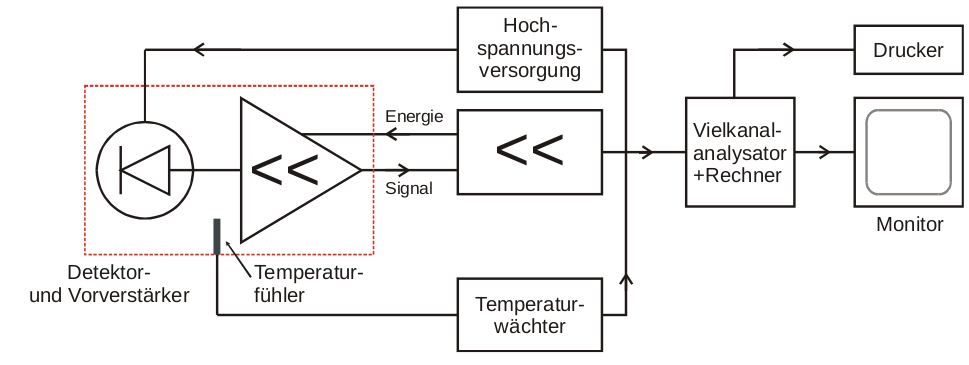
\includegraphics[width=0.95\textwidth]{blockschaltung.png}
  \caption{Blockschaltbild der elektrischen Schaltung. Der Temperaturwächter verhindert dass die Hochspannung
  an einen Detektor angelegt wird, der nicht ausreichend gekühlt ist \cite{anleitungv18}.}
  \label{fig:blockschaltbild}
\end{figure}

\subsection{Energiespektrum}

Das bei einem Germanium-Detektor enstehende Spektrum ist in Abb. \ref{fig:spektrum}
dargestellt. Von besonderem Interesse ist dabei der Photo- bzw. Vollenergiepeak, da
dieser die Photonen beschreibt die ihre gesamte Energie im Detektor deponieren.
Seine Halbwertsbreite ist die im vorherigen Kapitel beschriebene energetische Halbwertsbreite
$\Delta E_{1/2}$, und gibt daher Auskunft über die Auflösung des Detektors.
Das in Abb. \ref{fig:spektrum} zu sehende Compton-Kontinuum ist dagegen ein eher
unerwünschter Effekt, da bei diesem die Photonen nur einen Teil ihrer Energie deponieren.
Er besteht zum einen aus dem Rückstreupeak, welcher durch die Photonen ensteht die
nicht direkt in den Detektor gelangen. Damit sind vorallem die Photonen gemeint die
aus der Probe in einem hohen Winkel von dem Detektor weggestrahlt werden, und erst über mehrere
Wechselwirkungen mit der Umgebung in den Detektor gelangen. Zum Anderen besteht das
Kontinuum aus der Comptonkante. Diese bezeichnet das Ende des Kontinuums, und damit den
maximalen Energieübertrag des Comptoneffekts bei einem Streuwinkel von 180°. Der
maximale Energieübertrag beträgt dabei
\begin{align}
  E_{\symup{max}} = 2\varepsilon\,E_\gamma\,/\,(1+2\varepsilon).
\end{align}
Die geringe Intensität nach der Comptonkante ensteht durch mehrfache Comptonstreuung
von einem Photon.\\
\begin{figure}
  \centering
  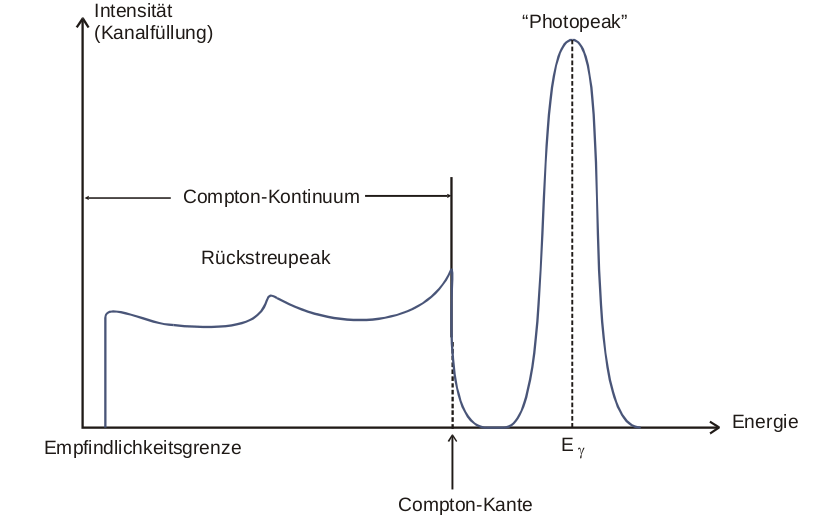
\includegraphics[width=0.95\textwidth]{spektrum.png}
  \caption{Intensität des von einem Germanium-Detektors aufgenommenen
   Energiespektrums  \cite{anleitungv18}.}
  \label{fig:spektrum}
\end{figure}

\noindent
Um die Messergebnisse des Detektors auslesen zu können muss eine Eichung erfolgen.
Aus dem aufgenommenen Spektrum eines bekannten Energiespektrums, lässt sich mittels einer linearen
Ausgleichsrechnung, eine Umrechnungsmöglichkeit von Kanalnummer auf Energie bestimmen.
Zusätzlich muss für die Eichung die zuvor erwähnte Effizienz Q des Detektors bestimmt werden.
Diese ergibt sich aus
\begin{align}
  \symup{Q} = 4\pi\,\cdot\symup{Z}\,(\Omega\cdot\symup{A}\cdot\symup{W})^{-1}.
\end{align}
Dabei steht W für die Emissionswahrscheinlichkeit einer bestimmten Photonenergie, Z für
die Summe der Impulse in einem aufgezeichneten Peak (aus Spektrum ablesbar), A für die
Aktivität des Strahlers und $\Omega$ für den Raumwinkel. Die Aktivität A muss aus den
Herstellungsangaben für den Strahler, und dem Zerfall des Nuklides bestimmt werden. Der
Raumwinkel $\Omega$ lässt sich aus
\begin{align}
  \Omega = 2\pi\,\left(1\,-\,\symup{a}\cdot(\symup{a}^2+\symup{r}^2)^{-\frac{1}{2}}\right)
\end{align}
berechnen, wobei der Abstand a von Probe zum Detektor groß gegenüber der Größe der Probe sein muss.
Der Radius r des Detektors lässt sich aus Abb. \ref{fig:detektor} ablesen.

Nach der durchgeführten Energieeichung lässt sich aus aufgenommenen Energiespektren
auf Aktivität und Nuklidart der Probe schließen.

\subsection{Versuchsdurchführung}

Für die Eichung wird als erstes für jeweils eine Stunde das bereits bekannte Energiespektrum eines
Europium- und Caesium-Strahlers aufgenommen. Anschließend wird ein Strahler für eine Stunde
aufgezeichnet, bei dem es sich entweder um Antimon oder Barium handelt. Es soll die Aktivität des
Strahlers ermittelt werden.
Zum Schluss wird zur Nuklidbestimmung ein gänzlich unbekannter Strahler gemessen.
